\section{Results}
%In the following paragraphs the results of the simulation study are presented and discussed with constant reference to the possible clinical application of the CLaRyS Compton camera system as particle therapy monitor. 
The possible implementation of the ClaRyS Compton camera as a monitoring system for ion beam therapy has been tested. The detection efficiency of the camera has been tested with the irradiation with point-like gamma sources in different position with respect to the center of the camera. The beam exposure has been simulated with different beam intensities for an analysis of the detection environment (background, random coincidence contamination) and the camera precision in the identification of the fall-off of the dose profile has been investigated. For this purpose, the comparison of two different reconstruction methods (line-cone analytical reconstruction and MLEM iterative algorithm) is presented. 


\subsection{Compton camera absolute efficiency}
\label{Results::efficiency}

The obtained results are shown in figure \ref{fig::efficiency_study}. On the left side, we show the results achieved with an ideal detector, while on the right side realistic energy cuts are applied on each detector section: the lower energy limit  has been set to 50~keV for the scatterer and 100~keV for the absorber.

\begin{figure} [!hbtp]	
\centering
\subfloat[]{\includegraphics[width=0.5\textwidth]{./Figure/EffVSpos.pdf}}
\subfloat[]{\includegraphics[width=0.5\textwidth]{./Figure/EffVSpos_withCut.pdf}}
\caption{Absolute Compton camera efficiency as a function of the gamma source position for different gamma energies, in the range between 300~keV to 6~MeV. The left side shows the camera efficiency without any applied energy cut. It models an ideal Compton camera. In the right side, detector energy cuts are applied: the lower energy thresholds are set to 
50~keV for the scatterer and 100~keV for the absorber, to reproduce realistic scenario. This values can change for the final detector configuration, according to the detector energy resolutions achieved.}
\label{fig::efficiency_study}
\end{figure}

As expected according to the interaction probability energy dependency, the efficiency is higher for low gamma energies, and it lies in the range $4\times10^{-4}$ at 300~keV and $1.5\times10^{-4}$ at 6~MeV (figure \ref{fig::efficiency_study}). Moreover, it can be noticed how the efficiency quickly drops quickly as the point source drifts away from the camera center: this effect is more important for high energies, for which the incident gamma is less deflected in the scatterer for the same energy deposited compared to a low energy gamma (see equation~\ref{Compton_equation}). Therefore, considering 1~MeV as the average and reference gamma energy for ion beam therapy monitoring, the Compton camera position optimization with respect to the expected Bragg peak position appears mandatory for an efficient fall-off reconstruction.\newline
Regarding the applied energy cuts, figure~\ref{fig::efficiency_study}(b) clearly shows an important effect on low energy gammas in the central area of the camera. The effect is negligible for positions with a distance greater than 200~mm from the center of the camera, and for any distance at energies above 2~MeV. A further study showed how this effect is mainly due to the cut applied on the scatterer detector. Indeed, for low energies, below 2~MeV, the increased efficiency in the central section of the camera active surface shown in figure~\ref{fig::efficiency_study}(a) is linked to the increased relative number of photons approaching the camera with small angles. These photons are more likely undergoing Compton scattering with a reduced energy deposition, which is recorded by an ideal detector and rejected by the energy cut. The effect is all the more important as the primary gamma energy is limited, creating the peculiar energy dependence of the efficiency reduction emerged in the results in figure~\ref{fig::efficiency_study}(b).
 

\subsection{Beam intensity}
\label{Results::beamInt}


 
In figure~\ref{fig:coincidences} the different components of the resulting secondary signal are shown as a function of the beam intensity. The true coincidences represent detector time coincidences generated by the same gamma ray. All the other coincidence types compose the background. All the simulations are performed with $10^{8}$ primary protons and  $2\times10^{5}$ primary carbon ions. Those value correspond to realistic clinical values used for the treatment of a single spot. The collected data sets are reported with and without the applied time-of-flight discrimination, mainly employed for neutron rejection, as mentioned in section~\ref{MatMeth::TOF_Ecut}.


\begin{figure} [!h]
  \subfloat[]{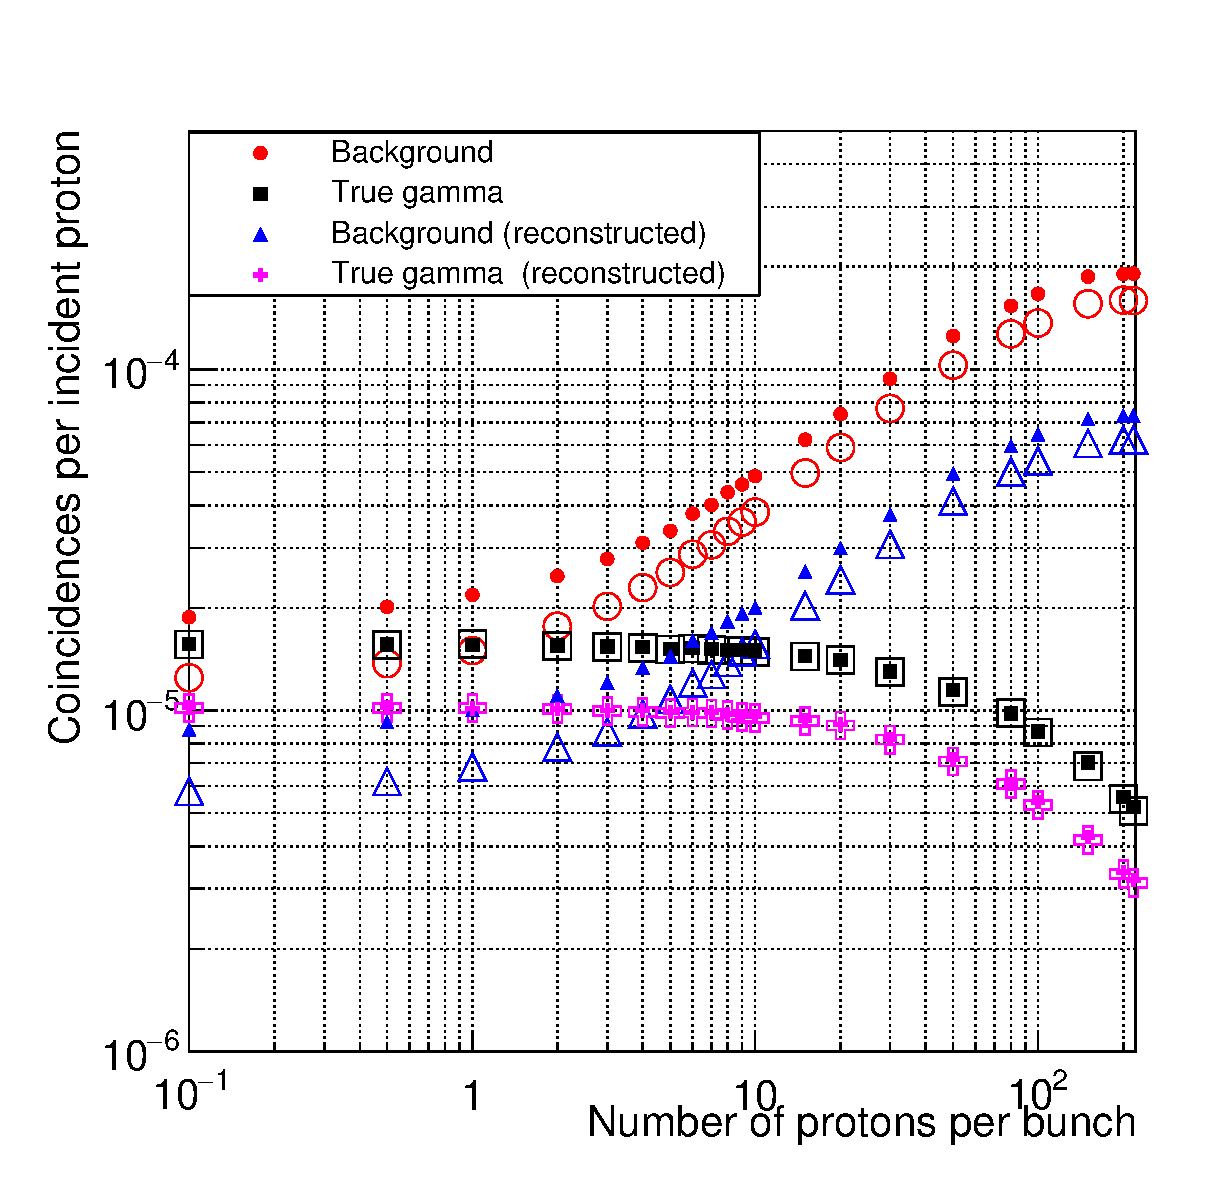
\includegraphics[width=0.5\textwidth]{./Figure/2017_06_28_Taux_coincidences_variation_protons_New_design_4EntreesLegend_LogXLogY.eps}}
  \subfloat[]{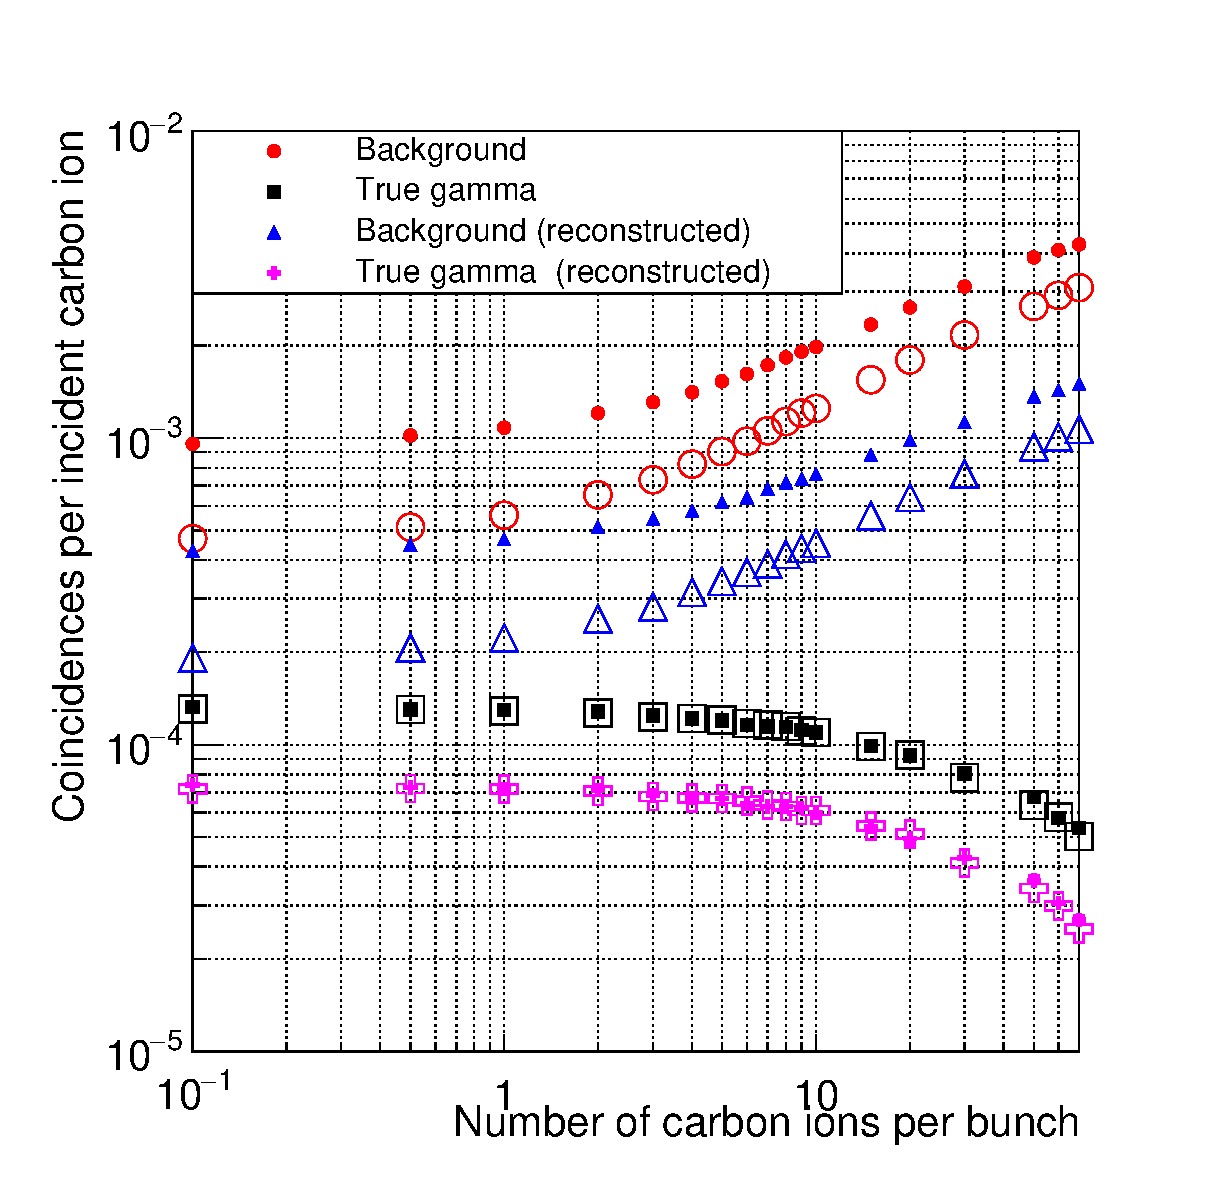
\includegraphics[width=0.5\textwidth]{./Figure/2017_06_28_Taux_coincidences_variation_carbonIons_New_design_4EntreesLegend_LogXLogY.eps}}
  \caption{Coincidences yield for protons (left) and carbon ions (right) as a function of the beam intensity. The intensity is reported as number of incident particles per bunch. The filled markers correspond to the collected data without time-of-flight discrimination, while this cut is applied to the data reported with empty markers. Moreover, the yields are given before and after the profile reconstruction with the line cone algorithm.}
  \label{fig:coincidences}
\end{figure}

In figure~\ref{fig:coincidences}(a) and (b) the amount of true gamma coincidences and background events are reported before and after reconstruction (the reconstruction algorithms select the events according to the chosen reconstruction parameters) as a function of the beam intensity for proton (a) and carbon ion (b) beams. In addition to this, for each curve realized with the complete collected data set, the related one realized after time-of-flight selection of events is sketched. All the curves have been normalized to the number of incident ions.\newline
As expected, the amount of background events (mainly random coincidences) increases with the increasing beam intensity: a factor of about 30 with respect to true gamma events is obtained for proton beams at clinical intensity (200 proton/bunch) with no event selection, while a factor more than two times higher is reported for carbon ions in the same conditions. Even if the time-of-flight selection can slightly improve this result by reducing the amount of background events, it is evident that such a beam intensity is not optimal for a proper monitoring. Furthermore, considering the rate of single interactions per detector, the results obtained by a preliminary analysis showed, as an example, a single rate of about 300~MHz on the absorber and 20~MHz on the first scatterer planes. These rates are not compatible with the detection rate capabilities of the detector read-out chains. As a result, it appears not possible to perform a valuable treatment monitoring with the CLaRyS Compton camera at a clinical beam intensity.\newline
Nevertheless, the monitoring objective becomes feasible in a reduced beam intensity scenario for proton irradiation. Figure~\ref{fig:coincidences}(a) shows how the amount of true gamma events and background events becomes compatible at the intensity of about 1 proton per bunch. In the case of carbon ions, the larger amount of secondary neutron produced during the patient treatment seems to require other background rejection methods in order to lead to an advantageous signal-over-background ratio.\\
\newline
Given the results presented in this paragraph, in the following the attention will be focused on proton beams at reduced intensities, with the aim of comparing the line-cone reconstruction and the MLEM reconstruction algorithm and to estimate the camera fall-off identification precision.

\subsection{Compton camera precision: comparaison LM-MLEM vs Line cone reconstruction}
\label{Results::precision_reconstruction}

The simulation setup shown in figure~\ref{fig:fig_setup_CC_simulation_Hadronth} has been implemented to test the line-cone analytic reconstruction method and compare it to the iterative LM-MLEM algorithm developed in Lyon by the CREATIS group~\cite{maxim_filtered_2014,hilaire_compton_2014}. A single data set has been collected, corresponding to the irradiation of the PMMA phatom with a proton 160~MeV monoenergetic beam, with a reduced intensity of 1 proton per bunch. A total of 10$^{10}$ protons has been simulated to define the reference Bragg peak, and then different sub-data sets have been extracted for the precision estimate at different statistics, as explained in section~\ref{MatMeth:precision}. 
Figure~\ref{fig:comparison} shows the results of the reconstruction of the data set obtained for the selection of 10$^8$ primary protons of 160~MeV, via the two reconstruction method already detailed before. To be noticed that the two reconstruction methods produce different results: the line-cone method is based on the beam direction information, so that it naturally produce a mono-dimensional image as result, while the MLEM method is able to reconstruct the prompt-gamma emission distribution in 3 dimensions. A projection along the beam direction is then extracted from the MLEM reconstructed image in order to allow a direct comparison.\\  

\begin{figure} [!h]
\subfloat[]{\includegraphics[width=0.5\textwidth]{./Figure/projection2D_Z_corr_r20.png}}
\subfloat[]{\includegraphics[width=0.5\textwidth]{./Figure/profileY_corr_r20.png}}\\
\subfloat[]{\includegraphics[width=0.5\textwidth]{./Figure/2015_02_16_Reconstruction_coinc_160MeVProton_TOF_6ns_file0to100_zoom.pdf}}
\caption{Line cone and LM-MLEM reconstruction for a 160~MeV proton beam, $10^{8}$ total incident protons. The beam intensity is 1 proton per bunch. The Compton camera is centered at the expected Bragg peak position, $y=+50 mm$. The time-of-flight event selection is applied on the collected data set. 20 iterations are performed for the MLEM reconstruction.\\
Figure (a) represents the MLEM reconstructed 2D image in the plan (x,y), parallel to the camera entrance surface. The position $x=0 mm$ corresponds to the center of the PMMA phantom and the y direction corresponds to the beam axis.  In figure (b) the mono-dimensional profile along the y axis is sketched. The profile peak is located at $y=+50 mm$. Figure (c) shows the profile obtained by means of line-cone algorithm for the same time-of.flight selected data.}
\label{fig:comparison}
\end{figure}


The analysis method described in section~\ref{MatMeth:precision} is applied to the different data set to retrieve the camera precision in the  dose profile falloff identification. The results are shown in figure~\ref{fig:precision}, where the two reconstruction methods are represented by different markers. \\

\begin{figure}[!hbtp]	
\centering
\caption{Compton camera precision for two different reconstruction algorithms: line-cone and LM-MLEM. The precision is shown as a function of the total number of incident protons, in the range $1\times10^{8}$ to $5\times10^{9}$. A linear fit is realized on the results in order to obtain the slope of the results (p1 parameter in legend). A logarithmic scale is used on both axes. }	
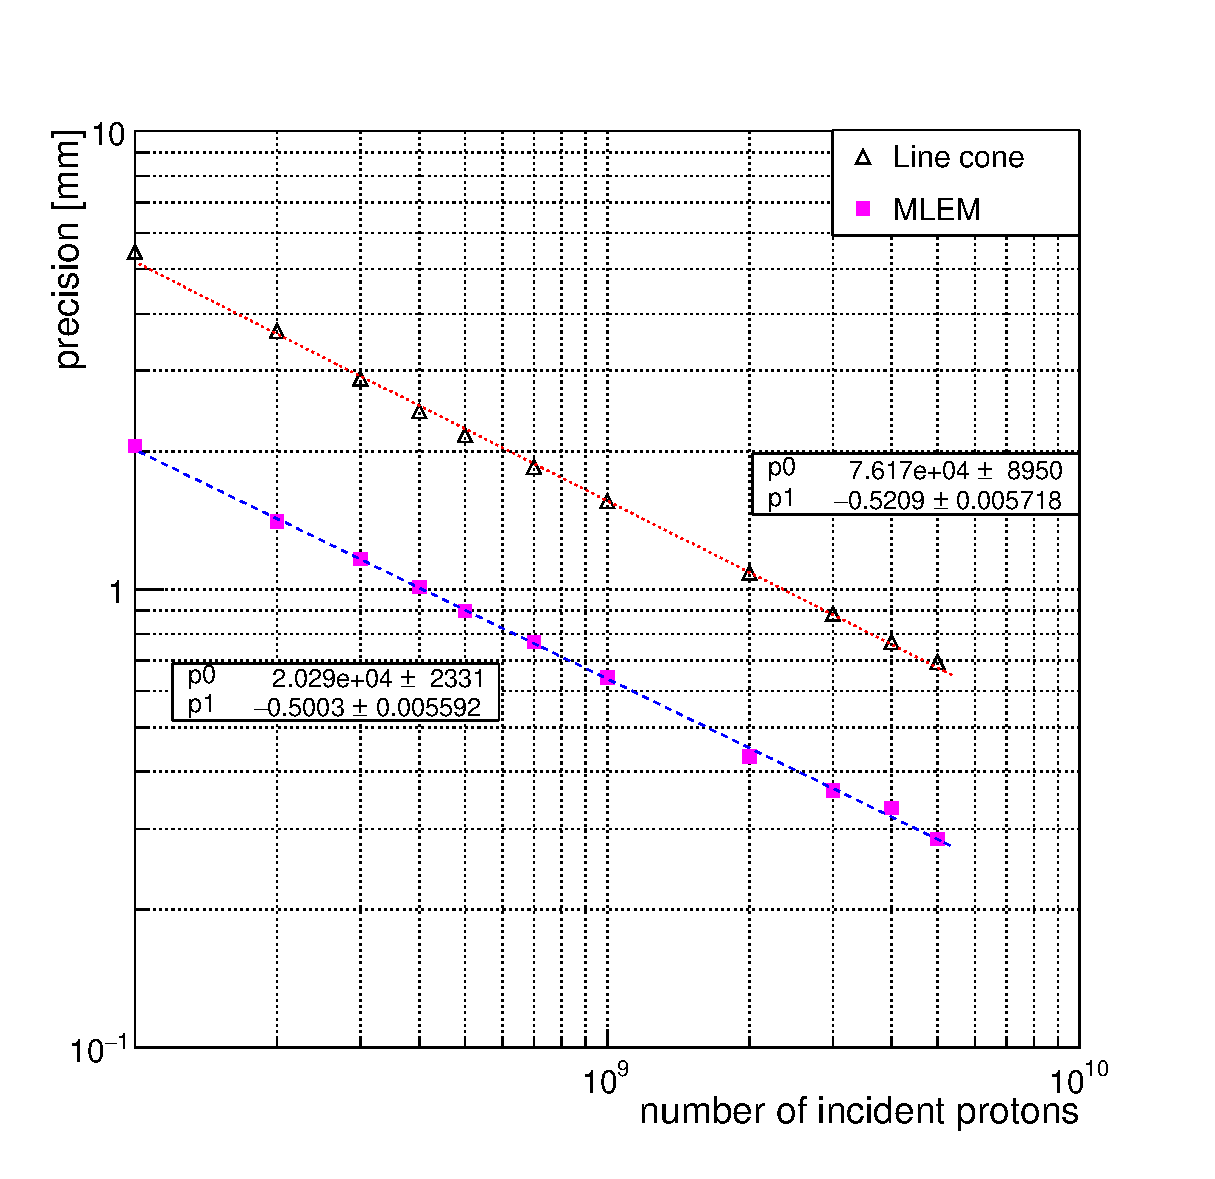
\includegraphics[width=0.7\textwidth]{./Figure/2017-10-21_Precision_Comparaison_linecone_MLEM_Article_Fit.eps}
\label{fig:precision}
\end{figure}

At the expense of an increased calculation time, the iterative MLEM reconstruction method allows to achieve a better precision, with a reduction of about 3~mm of the falloff retrieval precision in the whole range of statistics explored. A linear behavior, highlighted by the performed linear fit of the two data sets, is verified with increasing number of primary protons, starting from the single spot scale of about 10$^8$ primaries, till 5$\times$10$^9$ protons, which can correspond to the monitoring of a group of spot with the same planned range. If we consider the important increase in the precision of the falloff identification given by the increased statistics, the spot grouping method seems to be promising for monitoring purpose when high accuracy is required, probably obtained in the post-treatment due to the long required reconstruction time. A sufficiently good precision is achieved on a spot basis, where the precision is about 2~mm with a MLEM reconstruction: a qualitative monitoring of each spot seems then possible. Given the long calculation time required by the MLEM algorithm, the line-cone reconstruction method, despite the reduced precision, can still be an option for on-line treatment check, when safety limit can be fixed in order to exclude severe deviation from the treatment planning and an interruption of the dose delivery in real time can be foreseen.          


